% Accepted HISTORY1 results; data and drawing are owned by this figure project.
\begin{figure*}[t]
\centering
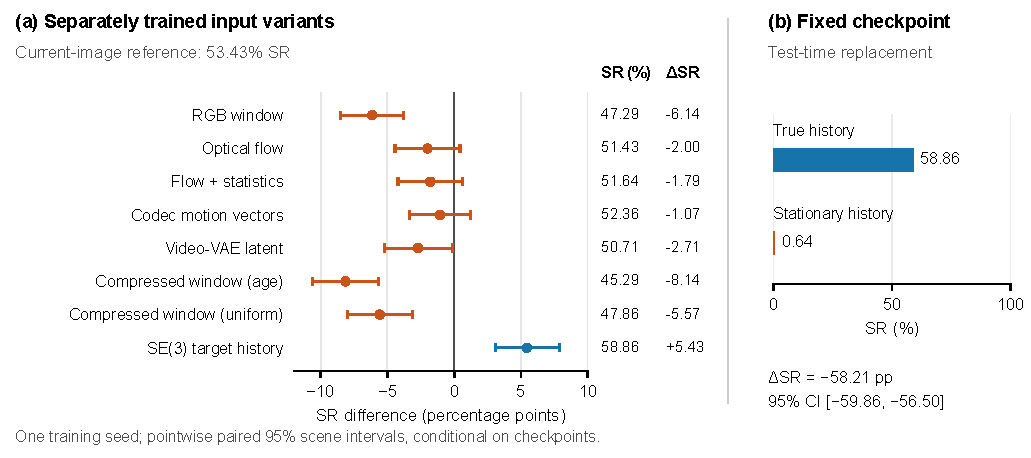
\includegraphics[width=\textwidth]{design_studies/history.pdf}
\caption{\textbf{History input and test-time intervention.} Frozen DINOv3-L, one training seed, 1{,}400 development scenes. All conditions retain the current GT target pose and robot history.
(a) Separately trained variants: SR and its difference from the current-image reference. Whiskers are pointwise paired 95\% scene-bootstrap intervals, conditional on trained checkpoints, without multiplicity adjustment.
(b) Replacing history at the same checkpoint: 824 versus 9 successes out of 1{,}400. This measures sensitivity to incorrect history, separately from the training benefit in (a).}
\label{fig:history_study}
\end{figure*}
